\documentclass{report}
\usepackage{graphicx}
\usepackage{listings}
\usepackage{xcolor}
\usepackage[a4paper, total={7in, 8in}]{geometry}
\usepackage{mdframed}
\usepackage[utf8x]{inputenc}
\usepackage[T1]{fontenc}
\RequirePackage[dutch,english]{babel}

\newmdtheoremenv{theo}{Theorem}

\definecolor{codegreen}{rgb}{0,0.6,0}
\definecolor{codegray}{rgb}{0.5,0.5,0.5}
\definecolor{codepurple}{rgb}{0.58,0,0.82}
\definecolor{backcolour}{rgb}{0.95,0.95,0.92}

\lstdefinestyle{mystyle}{
	backgroundcolor=\color{backcolour},   
	commentstyle=\color{codegreen},
	keywordstyle=\color{magenta},
	numberstyle=\tiny\color{codegray},
	stringstyle=\color{codepurple},
	basicstyle=\ttfamily\footnotesize,
	breakatwhitespace=false,         
	breaklines=true,                 
	captionpos=b,                    
	keepspaces=true,                 
	numbers=left,                    
	numbersep=5pt,                  
	showspaces=false,                
	showstringspaces=false,
	showtabs=false,                  
	tabsize=2
}
\lstset{style=mystyle}
\graphicspath{ {images/} }
\title{Databases II - Samenvatting Theorie, Hogent}
\author{SibianDG}
\date{\today}
\begin{document}
    \maketitle
    \tableofcontents
    \newpage
    
{\let\clearpage\relax \chapter{SQL : Review}}
    
    \begin{theo}[SQL bestaat uit 3 sub languages]

        \begin{itemize}
            \item \textbf{Data Definition Language} (DDL) 
            \item \textbf{Data Manipulation language} (DML)
            \item \textbf{Data Control Language} (DCL)
        \end{itemize}
    \end{theo}    

{\let\clearpage\relax \chapter{SQL : Advanced}}
    
    max aantal recursies = 100

{\let\clearpage\relax \chapter{SQL : Data Definition Language}}
    
    Fysieke opslag van data~\ref{fig:physicalStorageOfData}
    \begin{figure}
        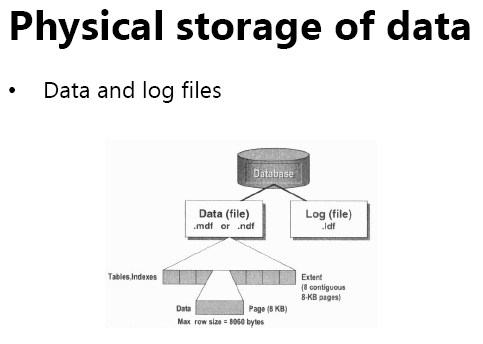
\includegraphics[width=350pt]{./images/storageData.png}
        \caption{\label{fig:physicalStorageOfData}Physical storage of Data}
    \end{figure}

    \subsection{Database maken}
    
   	\begin{itemize}
        \item Wie?
        \begin{itemize}
            \item sysadmin, use with "create database" permissions
        \end{itemize}
        \item Hoe?
        \begin{itemize}
            \item Een kopie van een "model" database wordt gemaakt
            \begin{itemize}
                \item de sysdatabases tabel in de Master database bevat informatie over elke database
            \end{itemize}
            \item Specificeer de fysieke opslagkarakteristieken bij het creëren (of wijzigen) van een database:
            \begin{itemize}
                \item naam van de database/transaction log files
                \item grootte van de database/transaction log files
                \item locatie van de database(.mdf)/transaction log files(.ldf)
            \end{itemize}
        \end{itemize}
    \end{itemize}

    \subsection{Veranderende kenmerken van een databank}
   	\begin{itemize}  
        \item Wat?
        \begin{itemize}
            \item Beheer van de groei van de gegevens en het logbestand
            \item De grootte van de gegevens en de logbestanden vergroten of verkleinen
            \item Toevoegen/verwijderen van secundaire gegevensbestanden, logbestanden
        \end{itemize}
    \end{itemize}

    \subsection{The CREATE TABLE command}
    \begin{itemize}  
        \item Bij het maken van een tabel specificeren we
        \begin{itemize}
            \item De naam van de tabel
            \item De definitie van de kolommen (naam, datatype)
            \item De definitie van de constraints
        \end{itemize}
    \end{itemize}

    \subsection{Scripts}
    \begin{itemize}  
        \item Scripts worden gebruikt voor
        \begin{itemize}
            \item Batchverwerking
            \item Creëren van test- en productieomgeving
        \end{itemize}
    \end{itemize}

    \subsection{Datatypes}
    \subsubsection{Categorieën van data types}
    \begin{center}
        \begin{tabular}{ |c|c|c| } 
            \hline
            Exacte numerieke tekens & Unicode-tekenreeksen\\ 
            Numerieke getallen bij benadering & Binaire tekenreeksen\\ 
            Datum en tijd & Andere gegevenstypen\\ 
            Character strings & \\
            \hline
        \end{tabular}
    \end{center}
    \begin{itemize}  
        \item Exact numeric values
        \begin{itemize}
            \item With decimal/numeric you specify the precision (total number of digits) and the scale (number of decimals)
            \item bit can also be threated as boolean
        \end{itemize}
        \item Approximative numeric values
        \begin{itemize}
            \item specify the precision with float: number of bits for the mantissa (1 - 53)
            \item float(24) is equivalent to SQL 92 real
            \item float(53) is equivalent to SQL 92 double precision
        \end{itemize}
        \item Date and time values
        \begin{itemize}
            \item The precision of datetime: 3.33 milliseconds
            \item The precision of smalldatetime: 1 minute
        \end{itemize}
        \item Character strings
        \begin{itemize}
            \item Char and varchar contain non-unicode characters ($2^8$ = ASCII)
            \item Use char if column data has a consistent length (e.g. national identification number)
            \item varchar varying length
            \item n -> 1 - 8000
            \item 
            \item nchar and nvarchar contain unicode characters (216 combinations)
            \item n -> 1 - 8000
        \end{itemize}
        \item Binary data
        \begin{itemize}
            \item Write photo to database (column photo = type varbinary(max)):
\begin{lstlisting}[language=SQL]
UPDATE players
SET photo=( SELECT *
FROM OPENROWSET(BULK N'C:\temp\beer.jpg', SINGLE_BLOB) AS img)
WHERE playerno=2;\end{lstlisting}
        \end{itemize}
        
    \end{itemize}

    \subsubsection{CONSTRAINTS}
    \begin{itemize}
        \item identity column contains
        \begin{itemize}
            \item unique value for each row
            \item System generated sequential values
            \item Only 1 identity column per table is allowed
            \item @@IDENTITY returns the last generated identity value
        \end{itemize}
    \end{itemize}

    \subsubsection{Data integrity}
    \begin{itemize}
        \item Types
        \begin{itemize}
            \item Domain integrity
            \item Entity integrity
            \item Referential integrity
        \end{itemize}
        \item Ensure through
        \begin{itemize}
            \item Database definitions: constraints, defaults and rules
            \item Procedures: client (programs) or server (triggers and stored procedures)
        \end{itemize}
        \item Always prefer constraints through data definitions if possible
        \begin{itemize}
            \item More secure than applications: constraints can't be bypassed
            \item Generally better performance
        \end{itemize}
        \item Constraints
            \begin{itemize}
                \item Restrictions to data
                \item When adding, updating or deleting rows constraints are checked
                \item Different types
            \end{itemize}
    \end{itemize}
    
        
    Different types of data integrity with contraints \ref{fig:typesItegrity}
    \begin{figure}
        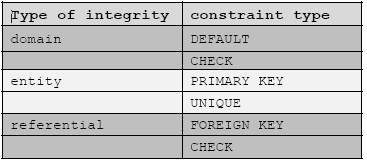
\includegraphics[width=250pt]{./images/typesItegrity.png}
        \caption{\label{fig:typesItegrity}Different types of data integrity with contraints}
    \end{figure}

    Please read all the contraints from slide 44
    
{\let\clearpage\relax \chapter{Window Functions}}

Geen theorie

{\let\clearpage\relax \chapter{Database programming}}
    PSM = Persistent Stored Modules
    
    Originally SQL was not a complete programming language
    
    SQL/PSM, as a complete programming language
    \linebreak
    variables, constants, datatypes, operators, Controle structures, procedures, functions, exception handling
    PSM = stored procedures and stored functions
    
    Examples: SQL Server: Transact SQL, Oracle: PL/SQL, DB2: SQL PL
    
    \bigskip
    \begin{theo}
    !!!! Procedural SQL extensions are vendor specific; database systems that use these extensions are more difficult to migrate to another RDBMS. !!
    \end{theo}
    \bigskip
    Proprietary languages!
    \bigskip
    \begin{theo}
    !! Besides views and CTE's, this is another way to reuse SELECT statements, now even parameterised !!
    \end{theo}

    \bigskip
    
    \subsection{Stored Procedures}
    Call in MS SQL Server:
    \linebreak \textendash exec DeleteCustomer 3000
    As DDL-element (table, index, view, \ldots) stored in the DB
    \linebreak
    
    \begin{theo}[Stored Procedure]
        A stored procedure is a named collection of SQL and control-of-flow
        commands(program)that is stored as a database object
    \end{theo}
    
    procedural database objects \ref{fig:proceduralDatabaseObjects}
    \begin{figure}
        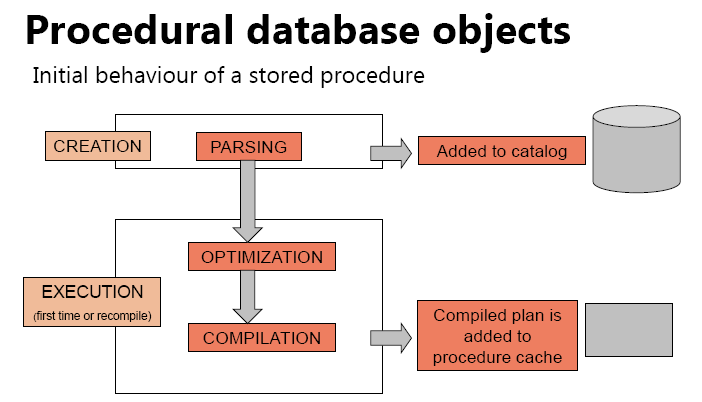
\includegraphics[width=400pt]{./images/proceduralDatabaseObjects.png}
        \caption{\label{fig:proceduralDatabaseObjects}procedural database objects}
    \end{figure}

    \subsection{Why using PSM's (SP and UDF)?}
    \subsubsection{PSM vs. 3GL (Java, .NET, C++, Cobol…)}
    \begin{itemize}
        \item Older versions of SQL Server (6.5 \& 7) and Oracle:
        \begin{itemize}
            \item Query-optimisation and execution plan caching \& reuse (see further) is better when using PSM
            \item SQL execution through PSM was more performant
        \end{itemize}
        \item Now: +/- same optimisation, no matter how query arrives at database
        \item Unfortunately performance is still used as a reason to use PSM's
    \end{itemize}

    \subsubsection{PSM: advantages}
    \begin{itemize}
        \item Code modularisation
        \begin{itemize}
            \item Reduce redundant code: put frequently used queries in SP and reuse in 3GL
            \item Less maintenance tasks at schema updates
            \item Often used for CRUD-operations
        \end{itemize}
        \item Customisation of "closed" systems like ERP: via stored procedures and triggers you can influence behaviour
        \item Security
        \begin{itemize}
            \item Exclude direct queries on tables
            \item SP's determine what is allowed
            \item Avoid SQL-injection attacks by using input parameters
        \end{itemize}
        \item Central administration of (parts of) DB code
    \end{itemize}

    \subsubsection{PSM-disadvantages}
    \begin{itemize}
        \item Reduced scalability: business logic and DB processing run on same server, can cause bottlenecks
        \item Vendor lock-in
        \begin{itemize}
            \item Syntax = non standard: port from ex. MS SQL Server to Oracle very time consuming
            \item But portability comes with a price (ex. built-in functions can't be used)
        \end{itemize}
        \item Two programming languages:
        \begin{itemize}
            \item JAVA/.NET/\ldots
            \item SP / UDF
        \end{itemize}
        \item Two debug environments
        \item SP/UDF: limited OO support
    \end{itemize}

    \subsection{Rules of thumb}
    \begin{itemize}
        \item Avoid PSM for larger business logic
        \item Consider using PSM for technical stuff
        \begin{itemize}
            \item Logging/auditing/validation
        \end{itemize}
        \item Make choice portability vs. vendor lock-in taking into account
        \begin{itemize}
            \item Your business departments.
            \item Corporate IT policies
        \end{itemize}
    \end{itemize}

    \subsection{Cursors}
    \begin{theo}[Cursor]
    SQL statements are processing complete resultsets and not individual rows. Cursors allow to process individual rows to perform complex row specific operations that can't (easily) be performed with a single SELECT, UPDATE or DELETE statement.
    \end{theo}
    A cursor is a database object that refers to the result of a query. It allows to specify the row from the resultset you wish to process.
    
    \subsection{Triggers}
        \begin{theo}[Trigger]
        A trigger:\\
        a database program, consisting of procedural and declarative instructons, saved in the catalogue and activated by the DBMS if a certain operation on the database is executed and if a certain condition is satisfied.
    \end{theo}
    Comparable to SP but can't be called explicitly
   \\
   A trigger is automatically called by the DBMS with some DML, DDL, LOGONLOGOFF commands

    trigger virtual table \ref{fig:triggerVirtualTable}
    \begin{figure}
        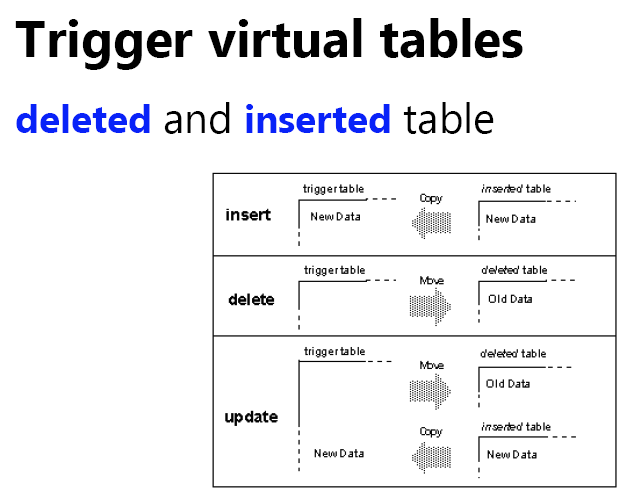
\includegraphics[width=400pt]{./images/triggerVirtualTable.png}
        \caption{\label{fig:triggerVirtualTable}trigger virtual table}
    \end{figure}

    \subsubsection{Creation of an after trigger}
    Only by SysAdmin or dbo
    Linked to one table; not to a view
    
    Overview Producural Database Objects \ref{fig:triggerVirtualTable}
    \begin{figure}
        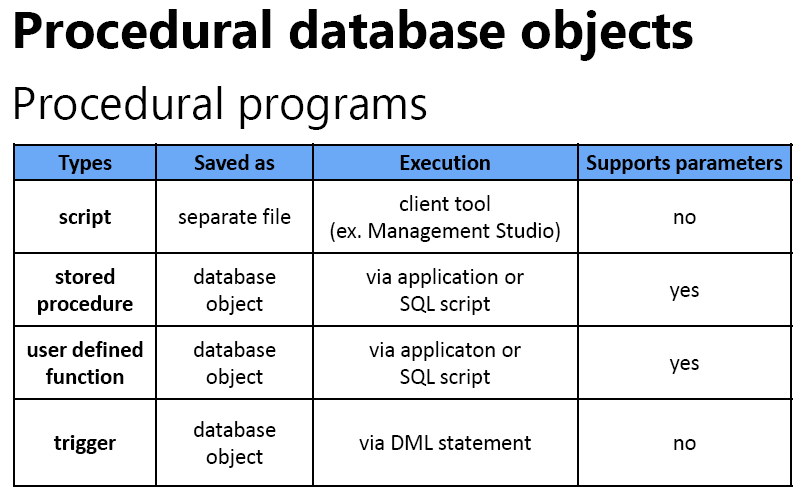
\includegraphics[width=300pt]{./images/ProducuralDatabaseObjects.png}
        \caption{\label{fig:ProducuralDatabaseObjects}ProducuralDatabaseObjects}
    \end{figure}
    
    \subsection{Why using triggers ?}
    \begin{itemize}
        \item Validation of data and complex constraints
        \begin{itemize}
            \item An employee can't be assigned to > 10 projects
            \item An employee can only be assigned to a project that is assigned to his department
        \end{itemize}
        \item Automatic generation of values
        \begin{itemize}
            \item If an employee is assigned to a project the default value for the monthly bonus is set  according to the project priority and his job category
        \end{itemize}
        \item Support for alerts
        \begin{itemize}
            \item Send automatic e-mail if an employee is removed from a project.
        \end{itemize}
        \item Auditing
        \begin{itemize}
            \item Keep track of who did what on a certain table
        \end{itemize}
        \item Replication and controlled update of redundant data
        \begin{itemize}
            \item DB xtreme: if an ordersdetail record changes, update the orderamount in the orders table
            \item Automatic update of datawarehouse tables for reporting (see "DWH")
        \end{itemize}
    \end{itemize}

    \subsection{Advantages and disadvantages}
    \begin{itemize}
        \item Major advantage
        \begin{itemize}
            \item Store functionality in the DB and execute consistently with each change of data in the DB
        \end{itemize}
        \item Consequences
        \begin{itemize}
            \item No redundant code
            \begin{itemize}
                \item Functionality is localised in a single spot, not scattered over different applications (desktop, web, mobile), written by different authors
            \end{itemize}
        \end{itemize}
        \item Written \& tested 'once' by an experienced DBA
        \item Security
        \begin{itemize}
            \item Triggers are in the DB so all security rules apply
        \end{itemize}
        \item More processing power
        \begin{itemize}
            \item For DBMS and DB
        \end{itemize}
        \item Fits into client-server model
        \begin{itemize}
            \item 1 call to DB-server: al lot can happen without further communication
        \end{itemize}
        \item Drawbacks
        \begin{itemize}
            \item Complexity
            \begin{itemize}
                \item DB design, implementation are more complex by shifting functionality from application to DB
                \item Very difficult to debug
            \end{itemize}
            \item Hidden functionality
            \begin{itemize}
                \item The user can be confronted with unexpected side effects from the trigger, possibly unwanted
                \item Triggers can cascade, which is not always easy to predict when designing the trigger
            \end{itemize}
            \item Performance
            \begin{itemize}
                \item At each database change the triggers have to be reevaluated
            \end{itemize}
            \item Portability
            \begin{itemize}
                \item Restricted to the chosen database dialect (e.g.: Transact-SQL from MS)
            \end{itemize}
        \end{itemize}
    \end{itemize}

    comparison of trigger functionality \ref{fig:comparisonTriggerFunc}\\
    \begin{figure}
        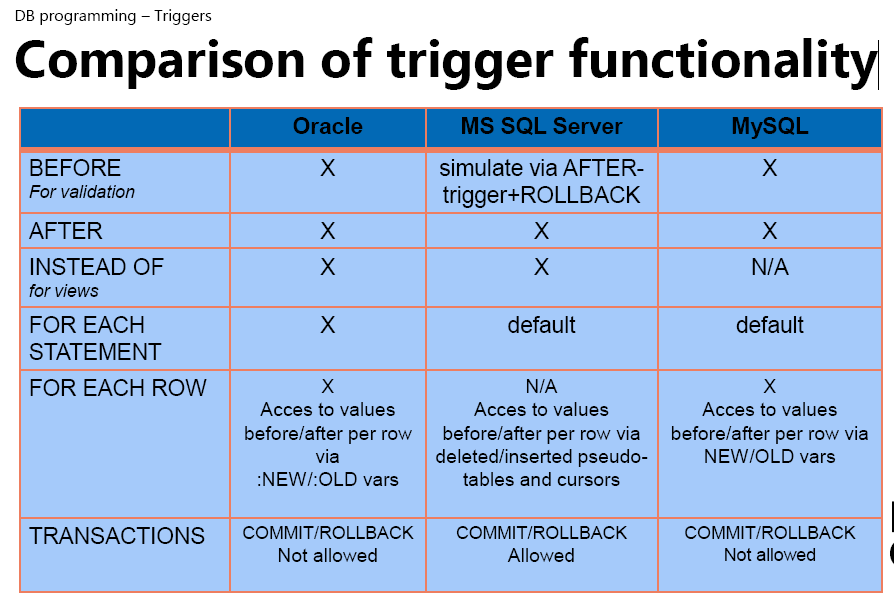
\includegraphics[width=350pt]{./images/comparison of trigger functionality.png}
        \caption{\label{fig:comparisonTriggerFunc}comparison of trigger functionality}
    \end{figure}

    \subsection{Tables and User Defined Types}
    \subsubsection{User defined types}
    \begin{itemize}
        \item ~Abstract data types
        \item Can be used as built-in types
        \item 2 sorts
        \begin{itemize}
            \item Distinct types
            \item Structured types: tables
        \end{itemize}
        \item Despite the SQL-2008-standard, many differences between DBMS's
    \end{itemize}
    
    \subsubsection{Distinct type}
    \begin{itemize}
        \item Based on a basic type
        \item Allows to refine existing data types
    \end{itemize}
    
\begin{lstlisting}[language=SQL]
CREATE TYPE IDType FROM INT NOT NULL;
CREATE TYPE NameType FROM NVARCHAR(50) NOT NULL;
\end{lstlisting}
    The new type is stored in the database\\
    The distinct type can be used as if it were a built-in type
    
    Remarks!\\
    \begin{itemize}
        \item ALTER TYPE [Name of the type] is not possible.
        \item DROP Type IDType;
    \end{itemize}

    \subsubsection{Table variables}
    \begin{itemize} 
        \item Local temporary tables
        \begin{itemize} 
            \item Stored in tempdb under "System Databases"
            \item Only visible:
            \begin{itemize} 
                \item In the creating session
                \item At the creating level
                \item In all underlying levels
            \end{itemize}
            \item Removed if creating level goes out-of-scope
        \end{itemize}
        \item Global temporary tables
            \begin{itemize} 
                \item Stored in tempdb under ``System Databases''
                \item Visible in all sessions
                \item Removed if creating session disconnects and there are no more references
            \end{itemize}
        \item Table Types and Variables
            \begin{itemize} 
                \item Table types are stored in the DB
                \item Table variables only exist during batch executions (= sequence of statements)
            \end{itemize}
            \begin{itemize} 
                \item Advantages of table variables and table types:
                \begin{itemize} 
                    \item Shorter and cleaner code
                    \item Table type variables can also be passed as parameters to stored procedures and functions
                \end{itemize}
            \end{itemize}
        \item Local temporary tables vs. table variables
            \begin{itemize} 
                \item Both are only visible in creating session
                \item Table variables have more limited scope:
                \begin{itemize} 
                    \item Only visible in current batch
                    \item Not visible in other batches in same session
                \end{itemize}
            \end{itemize}
    \end{itemize}

    \subsection{DYNAMIC SQL}
    \subsubsection{Early Binding versus Late Binding}
    \begin{itemize} 
        \item SQL binding refers to the translation of SQL code to a lower-level representation that can be executed by the DBMS, after performing tasks such as validation of table and field names, checking whether the user or client has sufficient access rights, and generating a query plan to access the physical data in the most performant way possible (see Chapter ``Indexes and Performance'').
        \item Early versus late binding then refers to the actual moment when this binding step is performed.
        \item Early binding is possible in case a pre-compiler is used and can hence only be applied with an embedded API
            \begin{itemize} 
                \item Beneficial in terms of performance
                \item Binding only needs to be performed on
                \item Pre-compiler can perform specific syntax checks
                \item Late binding performs the binding of SQL-statements at runtime
                    \begin{itemize} 
                        \item + Additional flexibility is offered ( ``dynamic SQL'')
                        \item - Syntax errors or authorisation issues will remain hidden until the program is executed
                        \item - Testing the application can be harder (use ``PRINT'')
                        \item Less efficient for queries that must be executed multiple times
                        \item Risk of SQL injection attacks (see further)
                    \end{itemize}
                \item Not allowed in UDF's (= risk of side effects)
            \end{itemize}
        \item Disadvantages:
            \begin{itemize} 
                \item No cached query execution plan -> slower
                \item Debugging is more difficult (use PRINT!)
                \item Not allowed in UDF's (= risk of side-effect)
                \item SQL injection
            \end{itemize}
    \end{itemize}
    \subsubsection{SQL Injection}
        \begin{itemize} 
            \item Never trust front-end data. Check for valid input (e.g.: only A-Z and 0-9 are allowed)
            \item Don't allow symbols like ' ; ( ) \textendash
            \item Pay attention if input data containing ``sp\_'' or ``xp\_'' -> these system stored procedures can be destructive
        \end{itemize}
    
{\let\clearpage\relax \chapter{Indexes and performance}}

    \section{Space allocation by SQL Server}
    \begin{itemize} 
        \item SQL Server uses random access files
        \item Page = 8 kB block of contiguous space
    \end{itemize}
    \section{Clustered vs. Non-clustered indexes}
    \subsection{Table scan}
    \begin{itemize} 
        \item Heap: unordered collection of data-pages without clustered index (see below) = default storage of a table
        \item Access via Index Alllocation Map (IAM)
        \item Table scan: if a query fetches all pages of the table -> always to avoid!
        \item Other performance issues with heap:
            \begin{itemize} 
                \item Fragmentation: table is scattered over several, non-consecutive pages
                \item Forward pointers: if a variable length row (e.g. varchar fields) becomes longer upon update, a forward pointer to another page is added. -> table scan even slower
            \end{itemize}
    \end{itemize}
    \subsection{What is the difference? Indexes!}
    \begin{itemize} 
        \item What?
            \begin{itemize} 
                \item Ordered structure imposed on records from a table
                \item Fast access through tree structure (B-tree = balanced tree)
            \end{itemize}
        \item Why?
            \begin{itemize} 
                \item Can speed up data retrieval
                \item Can force unicity of rows
            \end{itemize}
        \item Why not ?
            \begin{itemize} 
                \item Indexes consume storage (overhead)
                \item Indexes can slow down updates, deletes and inserts because indexes has to be updated too
            \end{itemize}
    \end{itemize}
    \subsection{SQL Optimizer}
        \begin{itemize} 
            \item SQL Optimizer: module in each DBMS
            \item SQL Optimizer: module in each DBMS
            \item Decides optimum strategy for e.g. index use based on statistics about table size, table use and data distribution
            \item In SQL searching is used for fields in where, group by, having and order by clauses and for fields that are joined
            \begin{itemize} 
                \item Fragmentation: table is scattered over several, non-consecutive pages
                \item Forward pointers: if a variable length row (e.g. varchar fields) becomes longer upon update, a forward pointer to another page is added. -> table scan even slower
            \end{itemize}
        \end{itemize}
    \subsection{Statistics}
    A cost-based optimizer uses statistics about tables, columns, and indexes. Most statistics are collected on the \textbf{column} level. The most important statistical value for a \textbf{table} is its size (in rows and blocks). The most important \textbf{index} statistics are: tree depth, number of leaf nodes, number of distinct keys. The optimizer uses these values to estimate the selectivity of the \textbf{WHERE} clause predicates
    \subsection{Clustered index}
        \begin{itemize} 
            \item The physical order of the rows in a table corresponds to the order in the clustered index.
            \item As a consequence, each table can have only one clustered index.
            \item The clustered index imposes unique values and the primary key constraint
            \item Advantages as opposed to table scan:
                \begin{itemize} 
                    \item Double linked list ensures order when reading sequential records
                    \item No forward pointers necessary
                \end{itemize}
        \end{itemize}
        Clustered index \ref{fig:clustered_index}
        \begin{figure}
            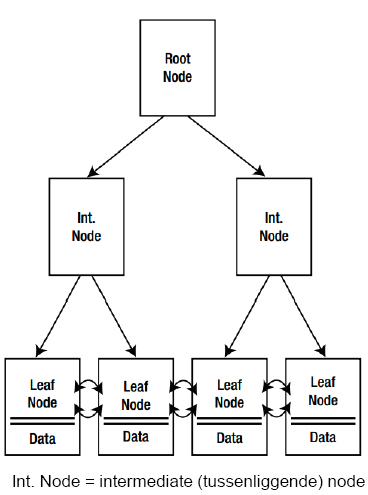
\includegraphics[width=180pt]{./images/clustered_index.png}
            \caption{\label{fig:clustered_index}Clustered index}
        \end{figure}
    \subsection{Non clustered index}
        \begin{itemize} 
            \item Default index
            \item Slower than clustered index
            \item > 1 per table allowed
            \item Forward and backward pointers between leaf nodes
            \item Each leaf contains key value and row locator
            \begin{itemize} 
                \item To position in clustered index if it exists
                \item Otherwise to heap
            \end{itemize}
            \item If the query needs more fields than present in index, these fields have to be fetched from data pages.
            \item When reading via non-clustered index:
                \begin{itemize} 
                    \item RID lookup = bookmark lookups to the heap using RID's (= row identifiers)
                    \item Key lookup = bookmark lookups to a clustered index, if present
                \end{itemize}
        \end{itemize}
        Non clustered index \ref{fig:non-clustered_index}
        \begin{figure}
            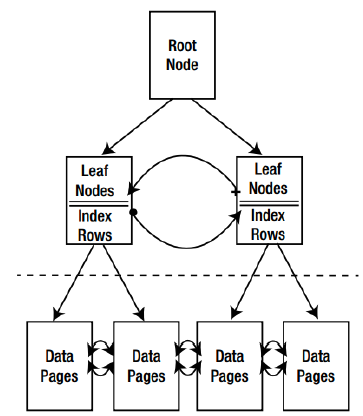
\includegraphics[width=180pt]{./images/non-clustered index.png}
            \caption{\label{fig:non-clustered_index}Non clustered index}
        \end{figure}
    \subsection{Use of indexes with functions and wildcards}
        \begin{itemize} 
            \item In the case of '\%r\%' (with a leading wildcard) the index can't be used for searching
            \item However, it may be advantageous to include the corresponding field in a covering index.
            \item That way, the data that is needed is “clustered” (= stored together), so fewer blocks have to be read.
        \end{itemize}
    \subsection{Covering index}
        \begin{itemize}
            \item If a non clustered index not completely covers a query, SQL Server performs a lookup for each row to fetch the data
            \item Covering index = non-clustered index containing all columns necessary for a certain query
            \item With SQL Server you can add extra columns to the index (although those columns are not indexed!)
        \end{itemize}
    \subsection{Concatenated Indexes}
        tja
    \subsection{Working with indexes}
        \subsubsection{Creation of indexes}
        \begin{lstlisting}[language=SQL]
            CREATE [UNIQUE] [| NONCLUSTERED]
            INDEX index_name ON table (kolom [,...n])
            
            create index ssnr_index on student(ssnr)
        \end{lstlisting}
        \begin{itemize}
            \item Unique: all values in the indexed column should be unique
            \item When defining an index the table can be empty or filled
            \item Columns in a unique index should have the not null constraint
        \end{itemize}
        \subsubsection{Removing indexes}
        \begin{lstlisting}[language=SQL]
            DROP INDEX table_name.index [,...n]
            
            drop index student.SSNR_Index
        \end{lstlisting}
    \subsection{Rules of thumb}
    \subsubsection{When to use an index}
    \begin{itemize}
        \item Which columns should be indexed?
            \begin{itemize}
                \item Primary and unique columns are indexed automatically
                \item Foreign keys often used in joins
                \item Columns often used in search conditions (WHERE, HAVING, GROUP BY) or in joins
                \item Columns often used in the ORDER BY clause
            \end{itemize}
        \item Which columns should not be indexed?
            \begin{itemize}
                \item Which columns should not be indexed?
                \item Columns that are rarely used in queries
                \item Columns with a small number of possible values (e.g. gender)
                \item Columns in small tables
                \item Columns of type bit, text of image
            \end{itemize}
    \end{itemize}
    \begin{enumerate}
        \item avoid the use of functions
        \item avoid calculations, isolate columns
        \item prefer OUTER JOIN above UNION
        \item avoid ANY and ALL
        \item Index for equality first — then for ranges
        \item Check the SQL code that is generated by your ORM tool or framework
        \item Avoid dynamic SQL whenever possible
        \item Use bind variables
        \item Execute joins in the database
        \item Avoid unnecessary joins
    \end{enumerate}

    \subsection{Quiz!!! Important}
    \subsubsection{Vraag 1}
        Is the following index a good fit for the query?
        \begin{lstlisting}[language=SQL]
        CREATE INDEX tbl_idx ON tbl (date_column);
        SELECT * FROM tbl
        WHERE YEAR(date_column) = 2017;
        \end{lstlisting}
    \begin{enumerate}
        \item Good fit: No need to change anything
        \item Bad fit: Changing the index or query could improve performance
    \end{enumerate}
    Bad fit: Je gebruikt een functie. De Where gebruikt de index niet.
    
    \subsubsection{Vraag 2}
        Is the following index a good fit for the query?
        \begin{lstlisting}[language=SQL]
        CREATE INDEX tbl_idx ON tbl (a, date_column);
        SELECT TOP 1 * FROM tbl
        WHERE a = 12
        ORDER BY date_column DESC;
        \end{lstlisting}
        \begin{enumerate}
            \item Good fit: No need to change anything
            \item Bad fit: Changing the index or query could improve performance
        \end{enumerate}
        Good fit: a en date-column komen voor in de index.
        
        
    \subsubsection{Vraag 3}
        Is the following index a good fit for both queries?
        \begin{lstlisting}[language=SQL]
        CREATE INDEX tbl_idx ON tbl (a, b);
        SELECT * FROM tbl
        WHERE a = 123 AND b = 1;
        SELECT * FROM tbl WHERE b = 123;
        \end{lstlisting}
        \begin{enumerate}
            \item Good fit: No need to change anything
            \item Bad fit: Changing the index or query could improve performance
        \end{enumerate}
        Bad fit: Omdat er bij de 2e select een vertraging gaat opzitten omdat er een combinatie is van A en B.
        
    \subsubsection{Vraag 4}
        Is the following index a good fit for the query?
        \begin{lstlisting}[language=SQL]
            CREATE INDEX tbl_idx ON tbl (text);
            SELECT * FROM tbl
            WHERE text LIKE 'TJ%';
        \end{lstlisting}
        \begin{enumerate}
            \item Good fit: No need to change anything
            \item Bad fit: Changing the index or query could improve performance
        \end{enumerate}
        Good fit: Het wordt niet aangeraden om indexen te maken voor tekstvelden, maar als je vaak selects hebt op tekstvelden waar je iets zoekt, gaat het toch enig nut hebben. Het gaat lang duren, maar zonder index gaat het nóg langer duren.
        
    \subsubsection{Vraag 5}
        This question is different.
        First consider the following index and query:
        \begin{lstlisting}[language=SQL]
        CREATE INDEX tbl_idx ON tbl (a, date_column);
        SELECT date_column, count(*) FROM tbl
        WHERE a = 123
        GROUP BY date_column;
        \end{lstlisting}
        Let's say this query returns at least a few
        rows.
        To implement a new functional
        requirement, another condition (b = 1) is
        added to the where clause:
        \begin{lstlisting}[language=SQL]
            SELECT date_column, count(*)
            FROM tbl
            WHERE a = 123 AND **b = 1**
            GROUP BY date_column;
        \end{lstlisting}
        How will the change affect performance:
        \begin{enumerate}
            \item Same: Query performance stays about the same 
            \item Not enough information: Definite answer cannot be given
            \item Slower: Query takes more time
            \item Faster: Query take less time
        \end{enumerate}
        Slower: er is extra kolom die je moet bekijken en zit niet in index en is te vergelijken.
        
{\let\clearpage\relax \chapter{Transactie management}}
    \section{Transactions, Recovery and Concurrency Control}
    \begin{itemize}
        \item set of database operations induced by a single user or application, that should be considered as one undividable unit of work
        \item Transaction always ‘succeeds’ or ‘fails’ in its entirety
        \item Transaction renders database from one consistent state into another consistent state
        \item Examples of problems: hard disk failure, application/DBMS crash, division by 0 ...
        \item Recovery: activity of ensuring that, whichever of the problems occurred, the database is returned to a consistent state without any data loss afterwards
        \item Concurrency control: coordination of transactions that execute simultaneously on the same data so that they do not cause inconsistencies in the data because of mutual interference
        \item Delineating transactions and the transaction lifecycle
        \item DBMS components involved in transaction management
        \item logfile
        \item Transactions boundaries can be specified implicitly
        or explicitly
            \begin{itemize}
                \item Explicitly: begin\_transaction and end\_transaction
                \item Implicitly: first executable SQL statement
            \end{itemize}
        \item Once the first operation is executed, the transaction is active
        \item If transaction completed successfully, it can be committed. If not, it needs to be rolled back.
    \end{itemize}
    \section{Logfile}
      Logfile registers unique log sequence number, unique transaction identifier, marking to denote the start of a transaction, along with the transaction’s start time and indication whether the transaction is
      read only or read/write, identifiers of the database records involved in the transaction, as
      well as the operation(s) they were subjected to, \textbf{before images} of all records that participated in the transaction, \textbf{after} images of all records that were changed by the transaction, the current state of the transaction (active, committed or aborted)
      \begin{itemize}
          \item Logfile may also contain checkpoints (moments when buffered updates by active transactions, as present in the database buffer, are written to disk at once)
          \item Write ahead log strategy
            \begin{itemize}
                \item all updates are registered on the logfile before written to disk
                \item before images are always recorded on the logfile prior to the actual values being overwritten in the physical database files
            \end{itemize}
      \end{itemize}
    \section{Recovery}
    \subsection{Types of Failures}
        \begin{itemize}
            \item \textbf{transaction} failure results from an error in the logic that drives the transaction’s
            operations and/or in the application logic 
            \item \textbf{System failure} occurs if the operating system or the database system crashes
            \item \textbf{Media failure} occurs if the secondary storage is damaged or inaccessible
        \end{itemize}
    \subsection{System Recovery}
    \begin{itemize}
        \item In case of system failure, 2 types of transactions
            \begin{itemize}
                \item already reached the committed state before failure
                \item still in an active state
            \end{itemize}
        \item Logfile is essential to take account of which updates  were made by which transactions (and when) and to  keep track of before images and after images needed for the UNDO and REDO
        \item Database buffer flushing strategy has impact on UNDO and REDO
    \end{itemize}
    \subsection{Media Recovery}
        \begin{itemize}
            \item Media recovery is invariably based on some type of data redundancy
            \item Tradeoff between cost to maintain the redundant data and time needed to restore the system
            \item Two types: disk mirroring and archiving
                \begin{itemize}
                    \item \textbf{Disk mirroring}: a (near) real time approach that writes the same data
                    simultaneously to 2 or more physical disks, limited failover time but often costlier than archiving, (limited) negative impact on write performance but opportunities for parallel read access
                    \item \textbf{Archiving}: database files are periodically copied to other storage media (e.g. tape, hard disk), trade-off between cost of more frequent backups and cost of
                    lost data, full versus incremental backup
                    \item \textbf{Mixed approach: rollfoward recovery}: Archive database files and mirror logfile such that the backup data can be complemented with (a redo of) the more recent transactions as recorded in the logfile
                    \item Note: NoSQL databases allow for temporary inconsistency, in return for increased performance (eventual consistency)
                \end{itemize}
        \end{itemize}
    \section{Concurrency Control}
    \begin{itemize}
        \item Scheduler is responsible for planning the execution of transactions and their operations
        \item Simple serial execution would be very inefficient
        \item Scheduler will ensure that operations of the transactions can be executed in an interleaved way
        \item Interference problems could occur: lost update problem, uncommitted dependency problem and inconsistent analysis problem
        
        \medskip
        
        \begin{itemize}
            \item \textbf{Lost update} problem occurs if an otherwise successful update of a data item by a transaction is overwritten by another transaction that wasn’t ‘aware’ of the first update
            \item If a transaction reads one or more data items that are being updated by another, as yet uncommitted, transaction, we may run into the \textbf{uncommitted dependency}/\textbf{dirty read} problem
            \item The \textbf{inconsistent analysis} problem denotes a situation where a transaction reads partial results of another transaction that simultaneously interacts with (and updates) the same data items.
            \item \textbf{nonrepeatable read (unrepeatable read)} occurs when a transaction T1 reads the same row multiple times, but obtains different subsequent values, because another transaction T2 updated this row in the meantime
            \item \textbf{phantom reads } can occur when a transaction T2 is executing insert or delete operations on a set of rows that are being read by a transaction T1
        \end{itemize}
    \end{itemize}
    \section{Schedules and Serial Schedules}
    \begin{itemize}
        \item \textbf{Schedule} S is serial if all statements si of the same transaction T are scheduled
        consecutively, without any interleave with statements from a different transaction
        \item Serial schedules prevent parallel transaction execution
        \item We need a non-serial, correct schedule!
        \item A \textbf{serializable} schedule is a non-serial schedule which is equivalent to a serial schedule
        \item A precedence graph can be drawn to test a schedule for serializability. If precedence graph contains a cycle, the schedule is not serializable.
        \item Scheduler applies scheduling protocol:
        \begin{itemize}
            \item Optimistic protocol
            \begin{itemize}
                \item conflicts between simultaneous transactions are exceptional
                \item transaction’s operations are scheduled without delay
                \item when transaction is ready to commit, it is verified for conflicts
                \item if no conflicts, transaction is committed. Otherwise, rolled back.
            \end{itemize}
            \item Pessimistic protocol
            \begin{itemize}
                \item it is likely that transactions will interfere and cause conflicts
                \item execution of transaction’s operations delayed until scheduler can schedule them in such a way that chance of conflicts is minimized
                \item will reduce the throughput to some extent
            \end{itemize}
        \end{itemize}
        \item Locking can be used for optimistic and pessimistic scheduling
        \begin{itemize}
            \item Pessimistic scheduling: locking used to limit the simultaneity of transaction execution
            \item Optimistic scheduling: locks used to detect conflicts during transaction execution
        \end{itemize}
        \item Timestamping
        \begin{itemize}
            \item Read and write timestamps are attributes associated with a database object
            \item Timestamps are used to enforce that a set of transactions’ operations is executed in the appropriate order
        \end{itemize}
    \end{itemize}
    
    \section{Locking and Locking Protocols}
    \begin{itemize}
        \item Purpose of locking is to ensure that, in situations where different concurrent transactions attempt to access the  same database object, access is only granted in such a way that no conflicts can occur
        \item A lock is a variable that is associated with a database object, where the variable’s value constrains the types of operations ththat are allowed to be executed on the object at that time
        \item Lock manager is responsible for granting locks (locking) and releasing locks (unlocking) by applying a locking protocol
        \item \textbf{An exclusive lock} (x-lock or write lock) means that a single transaction acquires the sole privilege to interact with that specific database object at that time (no other transactions are allowed to read or write it)
        \item A {shared lock} (s-lock or read lock) guarantees that no other transactions will update that same object for as long as the lock is held (other transactions may hold a shared lock on that same object as well, however they are only allowed to read it)
        \item If a transaction wants to update an object, an exclusive lock is required (only acquired if no other transactions hold any lock on the object)
        \item Compatibility matrix \ref{fig:Compatibility-matrix}
        \begin{figure}
            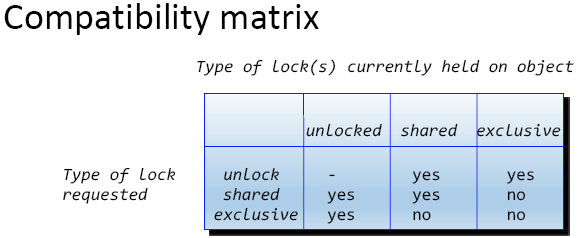
\includegraphics[width=220pt]{./images/Compatibility-matrix.png}
            \caption{\label{fig:Compatibility-matrix}Compatibility matrix}
        \end{figure}
        \item Lock manager implements locking protocol (set of rules to determine what locks can be granted in what situation (based on e.g. compatibility matrix ))
        \item Lock manager also uses a lock table (which locks are currently held by which transaction, which transactions are waiting to acquire certain locks, etc.)
        \item Lock manager needs to ensure ‘fairness’ of transaction scheduling to, e.g., avoid starvation        
    \end{itemize}
    \subsubsection{Two-Phase Locking Protocol (2PL)}
    \begin{itemize}
        \item Before a transaction can read (update) a database object, it should acquire a shared (exclusive) lock on that object
        \item Lock manager determines if requested locks can be granted, based on compatibility matrix
        \item Acquiring and releasing locks occurs in 2 phases
        \begin{itemize}
            \item growth phase: locks can be acquired but no locks can be released
            \item shrink phase: locks are gradually released, and no additional locks can be acquired
        \end{itemize}
        \item Variants: Rigorous 2PL: transaction holds all its locks until it is committed \&\& Static 2PL (Conservative 2PL): transaction acquires all its locks right at the start of the transaction
        \item Two-Phase Locking Protocol \ref{fig:2PL}
        \item Lost update problem with locking \& Uncommitted dependency problem with locking
        \item Revisit the uncommitted dependency problem
        \begin{itemize}
            \item problem is resolved if T2 holds all its locks until it is rolled back
            \item with 2PL protocol, locks can already be released before the transaction commits or aborts (shrink phase)
        \end{itemize}
    \item Cascading Rollback should be applied recursively
    \item -> best way to avoid this, is for all transactions to hold their locks until they have reached the ‘committed’ state (e.g., rigorous 2PL)
    \end{itemize}
    \begin{figure}
        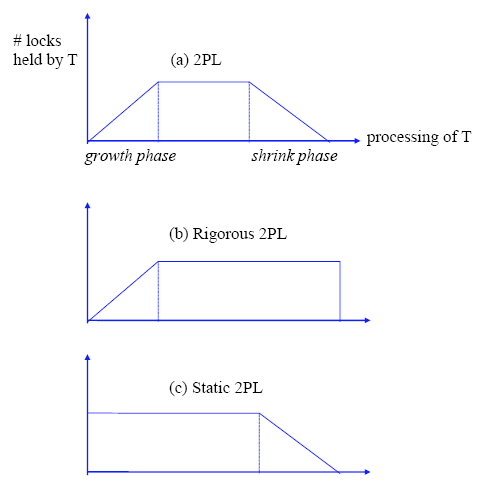
\includegraphics[width=240pt]{./images/2PL.png}
        \caption{\label{fig:2PL}Two-Phase Locking Protocol}
    \end{figure}
    \subsection{Dealing with Deadlocks}
    \begin{itemize}
        \item A deadlock occurs if 2 or more transactions are waiting for one another’s’ locks to be released
        \item Deadlock prevention can be achieved by static 2PL (transaction must acquire all its locks upon the start)
        \item Detection and resolution
        \begin{itemize}
            \item wait for graph consisting of nodes representing active transactions and directed edges Ti  -> Tj for each transaction Ti that is waiting to acquire a lock currently held by transaction Tj
            \item deadlock exists if the wait for graph contains a cycle
            \item victim selection
        \end{itemize}
    \end{itemize}
    \subsection{Isolation Levels}
    \begin{itemize}
        \item Level of transaction isolation offered by 2PL may be too stringent
        \item Limited amount of interference may be acceptable for better throughput
        \item Long-term lock is granted and released according to a protocol, and is held for a longer time, until the transaction is committed
        \item A short-term lock is only held during the time interval needed to complete the associated operation
        \item -> use of short-term locks violates rule 3 of the 2PL protocol \& can be used to improve throughput!
        \item \textbf{Read uncommitted}
        \item \textbf{Read committed}
        \item \textbf{Repeatable read}
        \item \textbf{Serializable}        
    \end{itemize}
    Isolation Levels \ref{fig:isolation-levels}
    \begin{figure}
        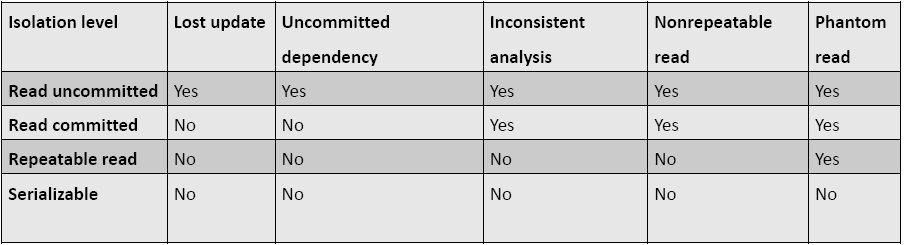
\includegraphics[width=350pt]{./images/isolation-levels.png}
        \caption{\label{fig:isolation-levels}Isolation Levels}
    \end{figure}
    \section{Lock Granularity}
    \begin{itemize}
        \item Database object for locking can be a tuple, a column, a table, a tablespace, a disk block, etc.
        \item Trade-off between locking overhead and transaction throughput
        \item Many DBMSs provide the option to have the optimal granularity level determined by the database system
    \end{itemize}
    \section{ACID Properties of Transactions}
    \begin{itemize}
        \item ACID stands for Atomicity, Consistency, Isolation and Durability
        \item \textbf{Atomicity} guarantees that multiple database operations that alter the database state can be treated as one indivisible unit of work
        \item \textbf{Consistency} refers to the fact that a transaction, if executed in isolation, renders the database from one consistent state into another consistent state
        \item \textbf{Isolation} denotes that, in situations where multiple transactions are executed concurrently, the outcome should be the same as if every transaction were executed in isolation
        \item \textbf{Durability} refers to the fact that the effects of a
        committed transaction should always be persisted into
        the database
    \end{itemize}
{\let\clearpage\relax \chapter{Datawarehousing \& Business Intelligence}}
    Knowledge piramid \ref{fig:knowledge-piramid}
    \begin{figure}
        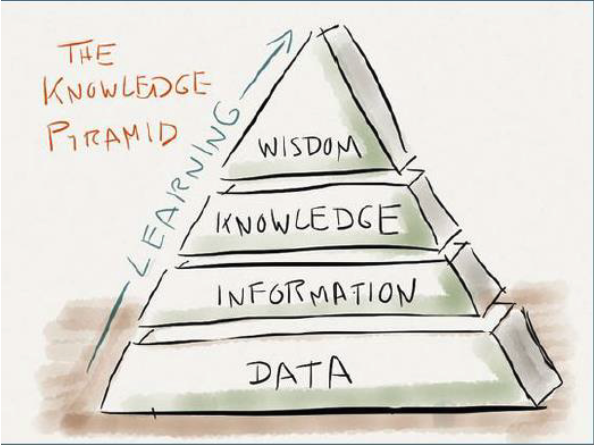
\includegraphics[width=200pt]{./images/knowledge-piramid.png}
        \caption{\label{fig:knowledge-piramid}Knowledge piramid}
    \end{figure}
    Business Intelligence (BI): Business intelligence, or BI, is a blanket term for technology that helps companies organize and query their data to help them improve operations and make more money.
    
    Drivers for increasing use of BI: Digitalisation(ERP, CRM), Connectors between BI software and Business software, Data overflow, Complexity and Speed of change in the Business Environment, Reduce inefficiencies, inaccuracies, Decreasing Cost
    
    Datawarehouse: A data warehouse is an integrated, subject oriented, time
    variant and non volatile collection of data to support decisions
    taken on management level.
    
    \subsection{Properties:}
    \begin{itemize}
        \item Subject oriented
        \item Integrated
        \item Time
        \item Non volatile
        \item Aggregated data
    \end{itemize}

    \subsection{Goals of DWH:}
    \begin{itemize}
        \item Reporting
        \item Analysis of events in the past or actual events
        \item Predictions based on trend analysis
        \item Multidimensional reporting
        \item Empowerment of end user by offering simplified reporting tools (cf. SQL: only specialist can write SQL)
        \item Data mining
    \end{itemize}

     \section{Advantages}
     \begin{itemize}
         \item High ROI (return on investment)
         \item Competitive advantage (Decision makers get access to data that was not available, unknown or unused before.)
         \item Increased productivity of corporate decision-makers
         \begin{itemize}
             \item Decision makers get one consistent view on the enterprise
             \item Decision makers can make more substantial, more accurate and more consistent analysis
         \end{itemize}
     \end{itemize}
 
    \section{Architecture}
    DWH components \ref{fig:dwh-components}
    \begin{figure}
        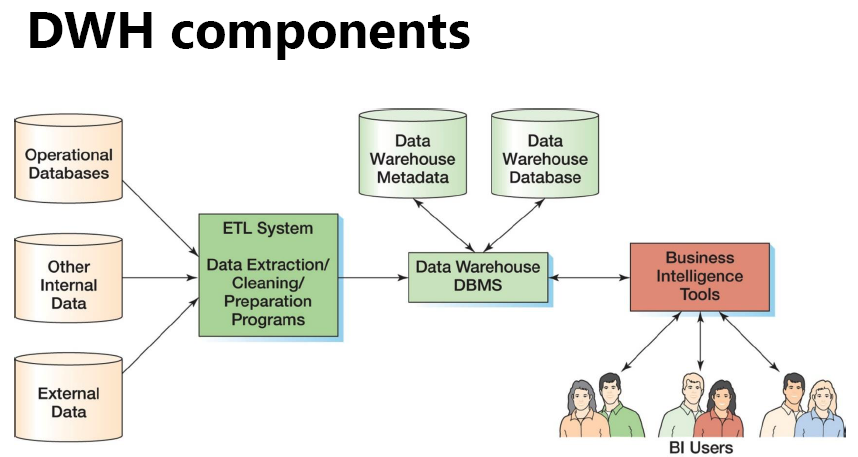
\includegraphics[width=250pt]{./images/dwh-components.png}
        \caption{\label{fig:dwh-components}DWH components}
    \end{figure}
    Read in slides
    
    \section{Datamart}
    A DB existing of a subset of company data to support the needs of a particular business unit for data analysis, or, to support users sharing the same needs for analyzing business processes.
    
    Why a data mart?
    \begin{itemize}
        \item To give users access to the data they analyse most frequently
        \item To offer data in a way that corresponds to the collective view of a group of users in a department or a group of users in the same business process
        \item To improve response time by offering lower data volumes
        \item To offer data in a format that fits the tools used by end users (OLAP, datamining tools)
        \item Reduction of complexity in the ETL process
        \item Reduction of cost as opposed to the setup of a complete DWH
    \end{itemize}
    \section{Data Mining Applications}
    \begin{itemize}
        \item Perform what-if analyses
        \item Perform predictions ("predictive analysis")
        \item Facilitate the decision process
    \end{itemize}
    \section{Problems associated with DWH}
    \begin{itemize}
        \item Underestimation of resources (costs) for ETL
        \item Hidden problems with source systems
        \item Required data not captured
        \item Increased end-user demands
        \item Data homogenization
        \item Need for concurrent support of several (historical) versions
        \item High demand for resources
        \item Data ownership
        \item High maintenance
        \item Long projects
        \item DWH creates expectation of user ‘empowering’: Make own reports, analyses
        \item Complexity of integration
        \item Complex change and version management
        \item -> Night might be too short for ETL
    \end{itemize}
    \subsection{Problems with Operational data}
    Dirty data, Missing values, Inconsistent data, Data not integrated, Wrong format, Too fine, Not fine enough, Too much data, Too many attributes, Too much volume
    
    \section{Design}
    \begin{itemize}
        \item Inmo
        \begin{itemize}
            \item Creation of a data model based on all data of the organisation
            \item Enterprise Data Warehouse (EDW)
            \item Used to distil data marts for each department
            \item Uses traditional methods for describing EDW
        \end{itemize}
        \item Kimball
        \begin{itemize}
            \item Starts by identifying the information requirements (referred to as analytical themes) and associated business processes of the enterprise -> Data Warehouse Bus Matrix; 
        \end{itemize}
    \end{itemize}

    \subsection{Star schema}
    A Star schema is a logical structure that 
    has a fact table (containing factual data) in the center, surrounded by denormalized dimension tables containing reference data).
    \begin{itemize}
        \item Fact table contains data about facts (E.g. factual data about sales of property: sales price, commission percentage)
        \item Dimension table contains reference informat (property data (address, etc), buyer, owner)
        \item Facts are generated by events that happened (e.g. a sale)
        \item Most probably facts never change
    \end{itemize}
    \subsection{Snowflake schema}
    Snowflake schema is a variant of the star schema that has a fact table in the centre, surrounded by normalised dimension tables.
    
    \subsection{Specific Schema Issues}
    \begin{itemize}
        \item Surrogate keys
        \begin{itemize}
            \item StoreKey, ProductKey, ShipperKey -> Meaningless integers
            \item Cannot use business keys since they usually have a business meaning
            \item Surrogate keys essentially buffer the data warehouse from the operational environment
            \item Business keys are usually bigger in size \& also often re-used over longer periods of time
        \end{itemize}
    \item Granularity of the fact table
        \begin{itemize}
            \item Level of detail of one row of the fact able
            \item Higher (lower) granularity implies more (fewer) rows
            \item Trade-off between level of detailed analysis and storage requirements
            \item example: One tuple of the fact table corresponds to one line on a purchase order
        \end{itemize}
    \end{itemize}
    \subsubsection{Factless Fact Tables}
    \subsubsection{Optimizing the dimension tables}
    Dimension tables should be heavily indexed to improve query execution time. average between 5 and 10 indexes. \textbf{time}: TimeKey, Date, DayOfWeek, DayOfMonth, DayOfYear
    
    Junk Dimensions: Deal with low cardinality attribute types such as flags or indicators. Eg. On-line Purchase (Y/N), Payment (cash or credit-card), Discount (Y/N)
    
    Outrigger tables: Store a set of attribute types of a dimension table which are highly correlated, low in cardinality and updated simultaneously.
    
    Slowly Changing Dimensions \& Rapidly changing dimensions
    
    \section{Advantages of the dimensional model}
    \begin{itemize}
        \item Efficiency
        \item Ability to handle changing requirements
        \item The model can easily adapt to changing needs because each dimension is equivalent to the fact table
        \item Extensibility
        \item Ability to model common business situations
        \item Predictable query processing
    \end{itemize}
    
    \section{Datawarehousing Delaware}
    Analytics. Data, analaytics, human input, decision, action.
    Met data kan je de kwaliteit van een proces verhogen. ERP maakt vb. veel data.
    
    \begin{enumerate}
        \item Connect/verbind
        \begin{itemize}
            \item verbinden van ongelijksoortige data: DB, cloud, app, big data, NoSQL, XML ...
        \end{itemize}
        \item Combine/combineer
        \begin{itemize}
            \item Datawarehouse: voorbereiden data
            \item connect: nomaliseren views ongelijksoortige data
            \item combineer: ontdek, transformeer, bereid voor, verbeter, kwaliteit, integreer
            \item publish: deel, lever, beheers en werk samen.
        \end{itemize}
        \item Verwerk/gebruik in business applicaties
        \begin{itemize}
            \item Data verwerkers/gebruikers: enterprise, rapporteren, analyse, BI
        \end{itemize}
    \end{enumerate}
    \subsection{Voordelen datawarehouse}
    \begin{itemize}
        \item Performantie
        \item betrouwbare data
    \end{itemize}
    Vb. van data \& DWH gebruiken: SAP groot touch screen live
    Use Case:Ze hadden betrouwbare informatie nodig!
    \begin{enumerate}
        \item Personal data
        \item Farm data
        \item Community data
    \end{enumerate}
\end{document}
